\chapter{Implementace systému}
% i tady, co tu popíšeme
% udělat do teoretický porovnámí yolov8 variant, čím a jak se liší, kolik používají vrstev atd, najít si zdroj.
% existuje program v latechu s názvem vlna
Tato kapitola popisuje praktickou realizaci navrženého dopravního monitorovacího systému a jeho softwarových komponent. V~první části je popsána konfigurace cílového linuxového prostředí, automatizace nasazení pomocí skriptů, oddělení citlivých údajů do proměnných prostředí a kontejnerizace referenčního i simulačního prostředí pomocí platformy Docker. Následuje detailní postup přípravy detekčního modelu \acs{YOLO} – od exportu vah do meziformátu \acs{ONNX} přes post-tréninkovou kvantizaci (\acs{PTQ}) do 8bitové celočíselné aritmetiky až po kompilaci do binárního souboru \acs{HEF} pro akcelerátor Hailo-8. Stěžejní část kapitoly se věnuje konstrukci multimediálního řetězce ve frameworku GStreamer, extrakci detekčních metadat ze snímkových bufferů, geometrickému vyhodnocování průjezdů knihovnou Shapely a implementaci asynchronního publikování událostí přes protokol \acs{MQTT} do databáze PostgreSQL a webového rozhraní ve frameworcích FastAPI a Streamlit.

\section{Konfigurace prostředí a automatizace běhu}
Pro praktickou realizaci systému na cílové platformě Raspberry Pi~5 byl nainstalován operační systém Raspberry Pi OS (založený na distribuci Debian Linux)~\cite{raspberrypi_docs_2024}, který poskytuje plnou podporu hardwarových rozhraní, dostupnost potřebných knihoven pro práci s~obrazem a sítí a kompatibilitu s~ovladači AI akcelerátoru Hailo-8. Řídicí skripty byly implementovány v~jazyce Python~3.11~\cite{python_docs_313_2025}.
%Implementace systému byla realizována v programovacím jazyce Python ve verzi 3.11 \cite{python_docs_313_2025}. 
%Python byl zvolen zejména díky:
%\begin{itemize}
%    \item široké podpoře knihoven pro počítačové vidění,
%    \item jednoduché integraci s databázovými systémy,
%    \item dostupnosti frameworků pro tvorbu webového API.
%\end{itemize}

\subsection{Automatická instalace závislostí a spouštění služeb}
Pro zajištění plné reprodukovatelnosti prostředí a snadného nasazení na nové zařízení byl vytvořen instalační skript, který automatizuje přípravu celého systému. Tento skript provádí:
\begin{itemize}
    \item instalaci systémových balíčků a multimediálního frameworku GStreamer,
    \item instalaci běhového prostředí HailoRT a knihoven TAPPAS~\cite{tappas_user_guide_331} pro AI akcelerátor,
    \item vytvoření virtuálního prostředí a instalaci Python knihoven (Ultralytics, Shapely, Paho-MQTT, Psycopg, FastAPI, Streamlit, Pandas, Plotly),
    \item nastavení systémových oprávnění a proměnných prostředí.
\end{itemize}

Aby byl zajištěn plně autonomní provoz systému v~reálných podmínkách (např. při výpadku napájení a následném restartu zařízení), byl v~operačním systému nakonfigurován spouštěcí mechanismus automatického spuštění hlavních služeb. Po inicializaci operačního systému spouštěcí skript nastaví potřebné proměnné prostředí a ve správném pořadí automaticky odstartuje hlavní komponenty:
\begin{enumerate}
    \item detekční pipeline běžící na edge zařízení,
    \item odběratelskou službu (MQTT subscriber) zajišťující zápis do databáze,
    \item backendový server (FastAPI) a webové vizualizační rozhraní (Streamlit).
\end{enumerate}

Tento přístup umožňuje plně autonomní provoz zařízení bez nutnosti manuálního zásahu po restartu systému. 

\subsection{Modularizace kódu, správa konfigurace a kontejnerizace (Docker)}
Pro zajištění udržitelnosti kódu a eliminaci duplicit mezi okrajovým zařízením (\texttt{rpi\_src/}) a referenční pracovní stanicí (\texttt{pc\_src/}) byla společná infrastruktura vyčleněna do sdíleného balíčku \texttt{common/}. Tento modul zapouzdřuje správu databázových spojení (\texttt{PostgreDatabaseManager}), komunikačního klienta (\texttt{MQTTPublisher}) a centralizované načítání konfigurace (\texttt{config.py}).

Z~hlediska kybernetické bezpečnosti jsou veškeré citlivé přihlašovací údaje (hesla k~databázi PostgreSQL, přístupové údaje k~MQTT brokeru a autentizační URL adresy RTSP kamerových toků) odděleny od zdrojového kódu a načítány dynamicky z~proměnných prostředí prostřednictvím souboru~\texttt{.env} (v~repozitáři je verzována pouze anonymizovaná šablona~\texttt{.env.example}).

Pro usnadnění replikovatelnosti experimentů a rychlé nasazení bez nutnosti manuální instalace závislostí byla implementována podpora kontejnerizace pomocí platformy \textbf{Docker} a nástroje \textbf{Docker Compose}:
\begin{itemize}
    \item \textbf{Kontejnerizované referenční prostředí (\texttt{pc\_src/docker-compose.yml}):} Definuje kompletní stoh služeb zahrnující databázi PostgreSQL (s~automatickou inicializací schématu pomocí skriptu \texttt{init\_hailo.sql}) a výpočetní kontejner s~akcelerací NVIDIA GPU pro běh referenčního detekčního skriptu.
    \item \textbf{Simulační prostředí (\texttt{rpi\_src/docker/}):} Umožňuje otestovat průchod dat celým řetězcem (od simulovaného publikování MQTT událostí přes databázovou vrstvu až po vykreslení ve webovém dashboardu) v~izolovaných kontejnerech i na zařízeních bez fyzicky připojeného akcelerátoru Hailo-8.
\end{itemize}

\section{Příprava a kompilace detekčního modelu}
\subsection{Volba varianty modelu a předzpracování}
%Pro detekci objektů byl zvolen model architektury YOLO (You Only Look Once), který je navržen pro real-time detekci objektů v jednom průchodu neuronovou sítí \cite{redmon_yolo_2016}. Modely YOLO jsou známé vysokým poměrem mezi přesností a rychlostí inference, což je klíčové pro nasazení na vestavěné edge platformě.

V~rámci implementace nebyl model trénován od začátku, ale byl využit předtrénovaný model rodiny YOLOv8 natrénovaný na datasetu COCO~\cite{lin_coco_2014}. Během vývoje byly experimentálně zkompilovány a otestovány varianty YOLOv8n, YOLOv8s a YOLOv8m, které se liší počtem parametrů. Pro finální nasazení byla zvolena varianta \textbf{YOLOv8m}, jež na cílové platformě vykazovala optimální kompromis mezi rychlostí inference a přesností detekce vzdálenějších vozidel.

Pro nasazení modelu na akcelerátor Hailo-8 lze buď využít předpřipravené modely z~repozitáře Hailo RPi5 Examples~\cite{hailo_rpi5_examples}, nebo provést vlastní kompilaci do binárního formátu HEF (\textit{Hailo Executable Format}) pomocí nástroje Hailo Dataflow Compiler (DFC)~\cite{hailo_dfc_docs}. V~této práci byl realizován kompletní proces vlastní kompilace. Před samotnou inferencí jsou vstupní snímky vždy převzorkovány na rozlišení $640 \times 640$ pixelů a převedeny do barevného formátu RGB.
%Model byl následně optimalizován a zkompilován pro běh na AI akcelerátoru Hailo pomocí nástroje Hailo Dataflow Compiler. Pro ověření funkčnosti modelu byla použita reálná data z dopravní kamery. Testovací sekvence obsahovaly vozidla různých tříd a byly zaznamenány za různých světelných podmínek.

\subsection{Export modelu do formátu ONNX}
Prvním krokem přípravy pro kompilátor Hailo DFC je převod vah modelu z~nativního formátu PyTorch (\texttt{.pt}) do standardizovaného meziformátu ONNX (\textit{Open Neural Network Exchange}). Export byl proveden pomocí knihovny Ultralytics s~pevně definovanou velikostí vstupu a zjednodušením výpočetního grafu (ukázka~\ref{lst:onnx_export}).

%ONNX představuje standardizovaný formát pro reprezentaci modelů neuronových sítí, který umožňuje interoperabilitu mezi různými frameworky pro strojové učení. Model YOLOv8 byl exportován z knihovny Ultralytics do formátu ONNX s velikostí vstupního obrazu 640×640 pixelů.

\begin{lstlisting}[language=Python, caption={Export modelu YOLOv8m do formátu ONNX.}, label={lst:onnx_export}]
from ultralytics import YOLO
model = YOLO("yolov8m.pt")
model.export(
    format="onnx",
    imgsz=640,
    opset=11,
    simplify=True
)
\end{lstlisting}

Výsledkem tohoto kroku je soubor \texttt{yolov8m.onnx}, který slouží jako přímý vstup pro optimalizační nástroje Hailo.

\subsection{Kvantizace a kompilace do formátu HEF}
Převod ONNX modelu do spustitelného formátu HEF byl proveden pomocí nástroje \texttt{hailomz} z~knihovny Hailo Model Zoo~\cite{hailo_model_zoo}. Tento proces zahrnuje čtyři fáze:
\begin{enumerate}
    \item překlad (parsing) ONNX grafu do meziformátu HAR (\textit{Hailo Archive}),
    \item optimalizaci a kvantizaci vah z~32bitové plovoucí řádové čárky (FP32) na 8bitová celá čísla (INT8),
    \item alokaci hardwarových výpočetních zdrojů cílového čipu,
    \item generování finálního binárního souboru HEF.
\end{enumerate}

Pro správné provedení post-tréninkové kvantizace (PTQ) do formátu INT8 vyžaduje kompilátor kalibrační sadu čítající řádově stovky až tisíce snímků, na kterých analyzuje statistické rozložení aktivací v~jednotlivých vrstvách. Pro tento účel byla využita validační část datasetu COCO (\texttt{val2017}) obsahující 5\,000 snímků~\cite{lin_coco_2014}. Vzhledem k~vysoké výpočetní a paměťové náročnosti procesu kompilace (který trvá v~řádu desítek minut) probíhal tento krok na externí pracovní stanici pomocí příkazu uvedeného v~ukázce~\ref{lst:hailo_compile}.

\begin{lstlisting}[language=bash, caption={Kompilace modelu YOLOv8m pomocí nástroje Hailo Model Zoo.}, label={lst:hailo_compile}]
hailomz compile yolov8m \
    --hw-arch hailo8 \
    --calib-path ./coco_val2017 \
    --classes 80
\end{lstlisting}

Vygenerovaný soubor \texttt{yolov8m.hef}, který je určen pro běh na architektuře Hailo-8, byl následně přenesen na zařízení Raspberry Pi~5, kde umožňuje provádět inferenci s~výrazně nižší latencí a spotřebou energie při zachování vysoké detekční přesnosti.

\section{Implementace zpracování videa a detekce}

\subsection{Konstrukce GStreamer pipeline}
Zpracování obrazového toku v~reálném čase je postaveno na zřetězení zásuvných modulů frameworku GStreamer. Pipeline se připojuje k~IP kameře přes protokol RTSP, provádí hardwarově či softwarově akcelerované dekódování komprimovaného formátu H.264, škáluje obraz na rozlišení $640 \times 640$ pixelů a předává jej specializovaným prvkům Hailo (ukázka~\ref{lst:gst_pipeline}).


\begin{lstlisting}[language=Python, caption={Zjednodušená konstrukce GStreamer pipeline.}, label={lst:gst_pipeline}]
pipeline_str = (
    "rtspsrc location=rtsp://CAMERA_IP latency=150 "
    "! rtph264depay ! h264parse ! avdec_h264 "
    "! videoconvert ! videoscale "
    "! video/x-raw,width=640,height=640,format=RGB "
    "! hailonet hef-path=yolov8m.hef batch-size=1 "
    "nms-score-threshold=0.6 nms-iou-threshold=0.5 "
    "! hailofilter function-name=yolov8m "
    "! hailotracker iou-thr=0.5 "
    "! videoconvert ! fakesink"
)
\end{lstlisting}

Samotnou inferenci na akcelerátoru zajišťuje prvek \texttt{hailonet}. Parametr \texttt{batch-size=1} garantuje, že každý přijatý snímek je zpracován okamžitě bez čekání na naplnění dávky více snímků, což minimalizuje latenci. Parametry \texttt{nms-score-threshold} a \texttt{nms-iou-threshold} konfigurují algoritmus \textit{Non-Maximum Suppression} (NMS), jenž filtruje detekce s~nízkou spolehlivostí a odstraňuje vícenásobné překrývající se rámečky nad stejným vozidlem. Následující prvek \texttt{hailofilter} provádí post-processing tenzorů a modul \texttt{hailotracker} přiřazuje objektům sledovací identifikátory na základě překryvu (\texttt{iou-thr=0.5}).

Pro účely ladění nebo paralelního ukládání záznamu lze pipeline na konci rozvětvit pomocí prvku \texttt{tee}, který duplikuje datový tok do více nezávislých větví a tím umožňuje paralelní zpracování výstupu z~pipeline, např. pro současné streamování a ukládání videa (ukázka~\ref{lst:gst_tee}).

\begin{lstlisting}[language=Python, caption={Větvení výstupu pipeline pomocí prvku tee.}, label={lst:gst_tee}]
pipeline_str += "! tee name=t "
pipeline_str += (
    "t. ! queue ! appsink name=rtsp_sink "
    "t. ! queue ! x264enc ! mp4mux ! filesink location=output.mp4"
)
\end{lstlisting}

Aby nedocházelo k~zahlcení paměti a postupnému narůstání zpoždění při případném kolísání výpočetního výkonu, jsou mezi klíčové fáze pipeline vloženy vyrovnávací fronty (\texttt{queue}), které oddělují jednotlivé fáze zpracování do samostatných vláken, s~aktivovaným režimem \texttt{leaky=downstream}. V~případě přetížení fronta automaticky zahodí nejstarší nezpracované snímky a upřednostní aktuální obraz z~kamery.

\subsection{Extrakce metadat pomocí Buffer Probe}
Aby nebylo nutné převádět celé obrazové snímky z~GStreameru do paměti Pythonu, je pro čtení výsledků detekce využit mechanismus \textit{buffer probe}. Na zdrojový výstup (\texttt{src} pad) prvku \texttt{hailotracker} je zaregistrována zpětná volací funkce (\textit{callback}), jež se automaticky spustí při průchodu každého snímku (ukázka~\ref{lst:buffer_probe}).

\begin{lstlisting}[language=Python, caption={Registrace buffer probe na výstupu sledovacího modulu.}, label={lst:buffer_probe}]
hailotracker = self.pipeline.get_by_name('hailotracker')
pad = hailotracker.get_static_pad('src')
pad.add_probe(Gst.PadProbeType.BUFFER, self.buffer_probe_callback)
\end{lstlisting}

Uvnitř callback funkce jsou pomocí Hailo API přímo z~paměťového bufferu GStreameru extrahovány objekty typu \texttt{HAILO\_DETECTION}, které nesou informaci o~detekované třídě, míře spolehlivosti, souřadnicích ohraničujícího obdélníku a přiděleném identifikátoru sledování (ukázka~\ref{lst:meta_extract}).

\begin{lstlisting}[language=Python, caption={Extrakce detekčních metadat z~GStreamer bufferu.}, label={lst:meta_extract}]
buffer = info.get_buffer()
roi = get_roi_from_buffer(buffer)
hailo_detections = roi.get_objects_typed(HAILO_DETECTION)

for detection in hailo_detections:
    label = detection.get_label()
    confidence = detection.get_confidence()
\end{lstlisting}

\subsection{Filtrace v~polygonální zóně (ROI) a eliminace duplicit}
Pro každé detekované vozidlo je nejprve vypočítán geometrický střed jeho ohraničujícího rámečku $(c_x, c_y)$. Pomocí geometrické knihovny \texttt{Shapely} je následně testováno, zda se tento bod nachází uvnitř uživatelsky definovaného polygonu oblasti zájmu (ukázka~\ref{lst:roi_shapely}).

\begin{lstlisting}[language=Python, caption={Filtrace detekcí v~definované polygonální ROI zóně.}, label={lst:roi_shapely}]
# Bounding box center determination
cx = bbox.xmin() + bbox.width() * 0.5
cy = bbox.ymin() + bbox.height() * 0.5

# Check if object is in zone
detection_point = Point(cx, cy)
if not self.zone_polygon.contains(detection_point):
    continue
\end{lstlisting}

Vzhledem k~tomu, že vozidlo projíždějící zónou ROI je zachyceno na desítkách po sobě jdoucích snímků, je nezbytné zabránit jeho opakovanému započítání. Aplikace si proto udržuje množinu již odeslaných identifikátorů \texttt{sent\_track\_ids}. Pokud se dané \texttt{tracking\_id} v~množině již nachází, je detekce přeskočena (ukázka~\ref{lst:dedup}).

\begin{lstlisting}[language=Python, caption={Prevence duplicitního odeslání téhož vozidla.}, label={lst:dedup}]
if tracking_id in self.sent_track_ids:
    continue

self._mark_sent(tracking_id)
\end{lstlisting}

Jelikož callback funkce GStreameru běží v~samostatném vlákně, je aktualizace sdílených stavových proměnných aplikace chráněna synchronizačním zámkem (\texttt{Lock}), čímž je zajištěna vláknová bezpečnost (\textit{thread-safety}):

\begin{lstlisting}[language=Python, caption={Vláknově bezpečná aktualizace detekčních dat.}]
with self.lock:
    self.detections = detections
    self.frame_count = frame_count
    self.timestamp = datetime.now().isoformat()
\end{lstlisting}

\subsection{Měření propustnosti (FPS)}
%Pro vyhodnocení schopnosti systému zpracovávat video stream v reálném čase byla implementována metrika Frames Per Second (FPS), která vyjadřuje počet zpracovaných snímků za sekundu.

%Výpočet FPS je realizován průběžně během běhu pipeline na základě počtu zpracovaných snímků a uplynulého času:

Pro průběžné sledování výkonnosti pipeline je přímo v~callback funkci implementován výpočet snímkové frekvence \acs{FPS} podle vztahu:
\[
\text{FPS} = \frac{N_{\text{frames}}}{t}
\]
kde $N_{\text{frames}}$ představuje celkový počet zpracovaných snímků od spuštění měření a $t$ je uplynulý čas v~sekundách (ukázka~\ref{lst:fps_calc}).

\begin{lstlisting}[language=Python, caption={Průběžný výpočet FPS během běhu pipeline.}, label={lst:fps_calc}]
self.frame_count += 1
elapsed_time = time.time() - self.start_time
fps = self.frame_count / elapsed_time
\end{lstlisting}

%Hodnota FPS je využívána jako indikátor výkonnosti celé detekční pipeline a umožňuje ověřit, zda systém splňuje požadavky na real-time zpracování. Díky využití hardwarového akcelerátoru je dosaženo stabilního průběhu zpracování bez významných výkyvů výkonu.

\section{Komunikace, ukládání a vizualizace dat}

\subsection{Publikace událostí přes MQTT}
Nově zaznamenané průjezdy vozidel zónou ROI jsou zformátovány do podoby slovníku, který obsahuje identifikátor a název třídy, míru spolehlivosti, souřadnice rámečku, sledovací ID a časové razítko. Pokud seznam obsahuje nové události a spojení s~MQTT brokerem je aktivní, data jsou serializována do formátu JSON a publikována do příslušného tématu (ukázka~\ref{lst:mqtt_pub}).

\begin{lstlisting}[language=Python, caption={Sestavení a publikace detekčních událostí přes MQTT.}, label={lst:mqtt_pub}]
detection_dict = {
    "class_id": class_id,
    "class_name": label,
    "confidence": float(confidence),
    "bbox": bbox_coords,
    "track_id": tracking_id,
    "timestamp": current_timestamp
}

detection_list.append(detection_dict)

if detection_list and self.mqtt_publisher.connected:
    self.mqtt_publisher.publish(detection_list)
\end{lstlisting}

Identifikátor \texttt{track\_id} je označen jako zpracovaný až v~okamžiku úspěšného předání zprávy komunikačnímu modulu, což zaručuje, že při případném krátkodobém výpadku spojení nedojde ke ztrátě detekce.

\subsection{Dávkové ukládání do databáze PostgreSQL}
%Pro ukládání detekčních událostí byl použit relační databázový systém PostgreSQL. Pro komunikaci mezi aplikací a databází byla využita knihovna Psycopg \cite{psycopg_docs_2025}.
%Detekční události jsou po přijetí prostřednictvím MQTT zpracovány a následně ukládány do relační databáze PostgreSQL.

Na serverové straně přijímá zprávy samostatný proces (MQTT subscriber). Pro zajištění vysoké propustnosti při komunikaci s~databází PostgreSQL využívá aplikace mechanismus \textit{connection poolingu} (opakované využívání otevřených databázových spojení). Samotný zápis dat do tabulky \texttt{detections} (jejíž schéma bylo definováno v~kapitole~\ref{fig:erd}) je realizován pomocí dávkového vkládání (\texttt{execute\_batch}) z~knihovny Psycopg, které umožňuje vložit až 100 záznamů v~rámci jediné databázové transakce (ukázka~\ref{lst:db_batch}).

\begin{lstlisting}[language=Python, caption={Dávkové vkládání detekčních záznamů do databáze PostgreSQL.}, label={lst:db_batch}]
query = """
INSERT INTO detections
(timestamp_, frame_id, class_name, confidence, x1, y1, x2, y2, track_id)
VALUES (%s, %s, %s, %s, %s, %s, %s, %s, %s)
"""
execute_batch(cursor, query, data, page_size=100)
conn.commit()
\end{lstlisting}

\subsection{Implementace vizualizačního dashboardu}
%Backendová část systému využívá framework FastAPI pro tvorbu REST rozhraní. Vizualizační vrstva je realizována pomocí frameworku Streamlit, který umožňuje rychlou tvorbu interaktivních dashboardů. Pro grafické výstupy byla použita knihovna Plotly \cite{plotly_docs_2015}.
Zpřístupnění uložených záznamů z~databáze PostgreSQL pro prezentační vrstvu zajišťují asynchronní \acs{REST} \acs{API} endpointy ve frameworku FastAPI (ukázka~\ref{lst:fastapi_endpoint}).

\begin{lstlisting}[language=Python, caption={Implementace REST API endpointu ve frameworku FastAPI pro čtení detekcí.}, label={lst:fastapi_endpoint}]
@app.get("/api/detections", response_model=List[DetectionResponse])
async def get_detections(minutes: int = 5, limit: int = 100):
    if db is None:
        raise HTTPException(status_code=503, detail="Database not initialized")
    detections = db.get_recent_detections(minutes=minutes, limit=limit)
    return [DetectionResponse(**dict(d)) for d in detections]
\end{lstlisting}

Uživatelské rozhraní vytvořené ve frameworku Streamlit (obrázek~\ref{fig:visualisation_dashboard}) načítá uložená data z~backendu (FastAPI framework) prostřednictvím \acs{REST} \acs{API} endpointů (\path{/api/detections} a~\path{/api/statistics}). Přijatá JSON data jsou převedena do struktury \texttt{DataFrame} knihovny Pandas, kde probíhá konverze časových razítek na typ \texttt{datetime}.

%Vizualizační rozhraní systému je realizováno jako interaktivní dashboard umožňující časovou analýzu detekcí, agregaci podle tříd objektů a prostorovou analýzu. Dashboard poskytuje přehled o celkovém počtu detekcí, průměrné hodnotě confidence a umožňuje volbu časového intervalu pro agregaci dat.

\begin{figure}[H]
    \centering
    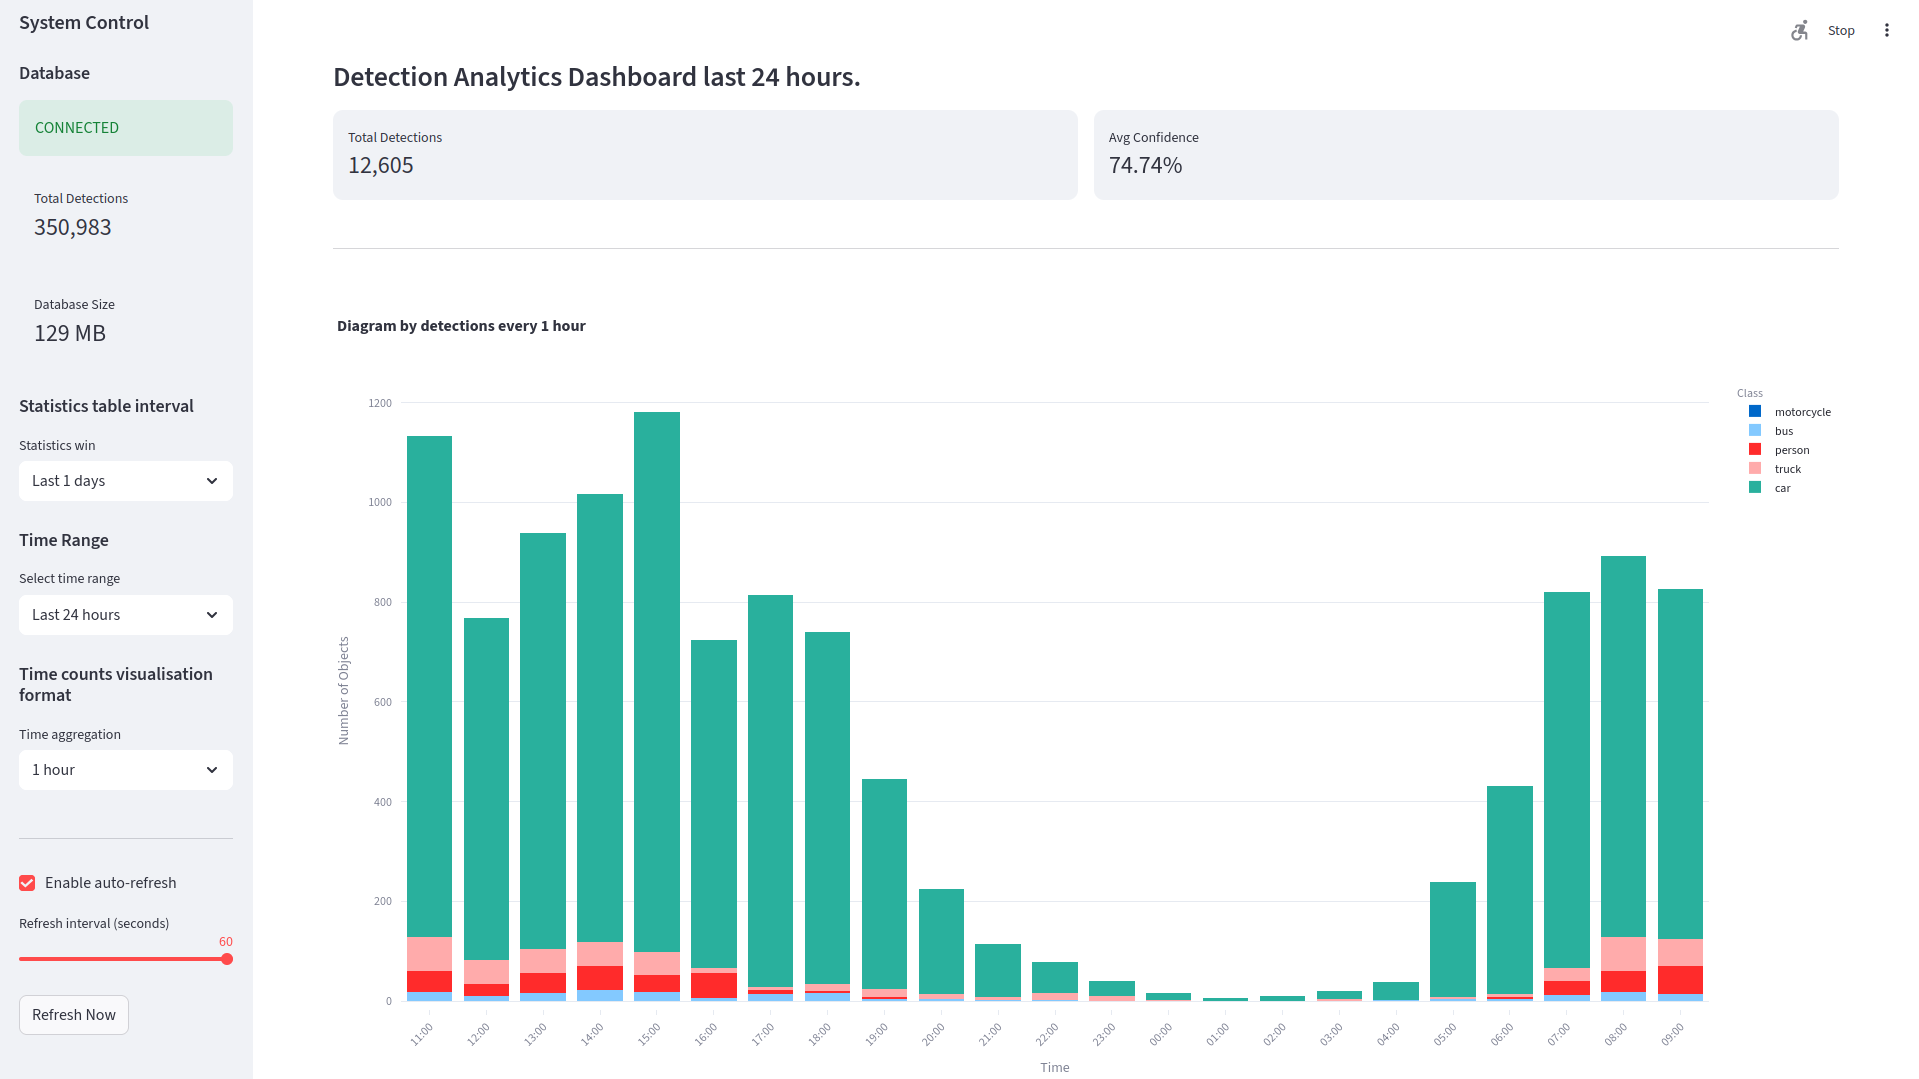
\includegraphics[width=0.95\textwidth]{images/visualisation_dashboard.png}
    \caption{Ukázka implementovaného vizualizačního dashboardu systému.}
    \label{fig:visualisation_dashboard}
\end{figure}

Pro dynamickou analýzu vývoje dopravy v~čase využívá aplikace metodu \texttt{resample()}, jež umožňuje uživateli měnit šířku časového okna agregace (např. 1~minuta, 10~minut, 1~hodina) jak globálně, tak pro jednotlivé kategorie vozidel (ukázka~\ref{lst:pandas_resample}).

\begin{lstlisting}[language=Python, caption={Časová agregace detekcí podle tříd vozidel v~knihovně Pandas.}, label={lst:pandas_resample}]
df_timeline = df.set_index("timestamp")

df_class_timeline = (
    df_timeline.groupby('class_name')
    .resample(selected_interval)
    .size()
    .reset_index(name="count")
)
\end{lstlisting}

%Tento přístup umožňuje dynamickou změnu velikosti časového intervalu a poskytuje flexibilní nástroj pro analýzu dopravní zátěže v různých časových měřítkách.

Agregovaná časová řada je následně vykreslena pomocí knihovny Plotly jako skládaný sloupcový graf (\textit{stacked bar chart}), který přehledně zobrazuje celkovou intenzitu provozu i poměrné zastoupení jednotlivých typů vozidel v~daných časových intervalech (ukázka~\ref{lst:plotly_bar}).

\begin{lstlisting}[language=Python, caption={Generování skládaného sloupcového grafu pomocí knihovny Plotly.}, label={lst:plotly_bar}]
fig = px.bar(
    df_class_timeline,
    x="timestamp",
    y="count",
    color="class_name",
    barmode="stack"
)
\end{lstlisting}
